% !TeX spellcheck = it_IT

\section{Altri esempi}

\addcontentsline{toc}{subsection}{\protect\numberline{}Nascita della teoria dei grafi}
\subsection*{Nascita della teoria dei grafi}

La città di K\"onigsberg è attraversata dal fiume Pregel, nel quale sono presenti due isole collegate da 7 ponti in totale.\\

La domanda posta ad Eulero fu: si può passare da tutti i ponti e tornare all'inizio? Ovvero, esiste un cammino che passa per tutti gli archi (ponti) del grafo per poi tornare al nodo iniziale?\\

Le due isole diventano 2 vertici e le sponde altri 2. Al giorno d'oggi sarebbe chiamato "multigrafo", avendo più lati incidenti sugli stessi due vertici, ma il problema rimane lo stesso.\\

Se volessimo formalizzare il problema nella terminologia moderna: dato un multigrafo, esiste un circuito che passa per tutti i lati? Si chiama "circuito Euleriano" (indovina perché).\\

\addcontentsline{toc}{subsubsection}{\protect\numberline{}Teorema di Eulero}
\paragraph{Teorema di Eulero:} \textbf{Esiste} un \textbf{circuito Euleriano iff} il grafo è connesso (ovviamente) e \textbf{tutti i vertici hanno grado pari}.\\

Come si \textbf{costruisce un circuito}, a partire \textbf{da un grafo con vertici di grado pari}? \\
Partendo da un qualsiasi vertice $x_0$ e si percorre un qualunque lato, arrivando ad $x_1$, il quale avrà almeno un altro lato uscente (avendo esso grado pari), che arriva ad $x_2$, e la cosa si ripete.\\
Nel caso si crei un ciclo prima di toccare tutti i lati vuol dire che questo ha almeno 4 lati incidenti e quindi si può continuare.\\
Se si torna ad $x_0$ prima di toccare tutti i lati, si ricomincia senza considerare i lati già visti.\\

\newpage

\addcontentsline{toc}{subsection}{\protect\numberline{}Handshaking Lemma}
\subsection*{Handshaking Lemma}
"Lemma delle strette di mano", se un gruppo di persone si stringono la mano, il numero di persone che stringono la mano ad un numero dispari di persone sono in quantità pari.\\

\addcontentsline{toc}{subsubsection}{\protect\numberline{}Teorema}
\paragraph{Teorema:} In un grafo $G=(V,E)$, il numero di vertici di grado ($d()$) dispari è pari.\\

\begin{proof}
	Sommando i gradi di tutti i vertici
	$$ \sum_{x \in V} d(x) = 2m $$
	In questo modo ogni lato viene contato 2 volte, quindi è pari 2 volte il nnumero di lati $m$. $2m$ è ovviamente pari, ed i nodi con grado pari possono non essere considerati ai fini della parità (se tolgo o aggiungo un numero pari la parità non cambia), quindi i nodi con grado dispari devono essere pari, altrimenti la somma potrebbe non essere pari.\\
\end{proof}

% End L9

\newpage

\subsection{Problema del Traveling Salesman (TSP)}
Avendo un insieme di città collegate da strade bidirezionali (grafo pesato) un commesso vuole passare per tutte le città una ed una sola volta, facendo un percorso di lunghezza minima per poi tornare a casa (vuole fare il giro).\\

Definizione: 
\begin{itemize}
	\item \textbf{Input}: un \textbf{grafo non orientato} $G = (V,E)$ con delle \textbf{lunghezze} $[\delta_e]_{e \in E}$ per ogni \textbf{lato}
	
	\item \textbf{Soluzioni ammissibili}: circuiti che passano per ogni vertice esattamente una volta (\textbf{circuito hamiltoniano})
	
	\item \textbf{Funzione obiettivo}: la \textbf{lunghezza} del circuito
	
	\item \textbf{Tipo}: minimizzazione, $\min$
\end{itemize}


Non è detto che il circuito hamiltoniano esista.\\

Questo problema è \textbf{equivalente al TSP su clique} (quindi su un grafo fully connected). Per usare un algoritmo che funziona solo su clique per grafi generici basta aggiungere i lati mancanti con un peso molto alto (più di ogni possibile cammino tra lati tendenzialmente), in modo che non vengano mai scelti, se la soluzione passa per uno dei lati "finti" nel grafo originale non c'è un circuito hamiltoniano.\\

Per questo da qui in poi verrà \textbf{presupposto che i grafi siano clique} $G = K_n$ (notazione per una clique di $n$ nodi).\\

\newpage

\paragraph{TSP Metrico:} Un TSP Metrico ha come proprietà:
\begin{itemize}
	\item $G$ è una clique 
	\item $\forall x,y,z$, $\delta_{xy} \leq \delta_{xz} + \delta_{zy}$ (disuguaglianza triangolare)
\end{itemize}

\nn

\paragraph{Ingredienti mancanti: } Due concetti che serviranno per l'algoritmo vero e proprio:
\begin{itemize}
	\item \textbf{Minimum spanning tree}: dato un grafo pesato connesso $G = (V,E)$ trovare un albero di copertura (che tocca tutti i vertici) di peso totale minimo. Risolvibile in tempo polinomiale (es. Algoritmo di Kruskal).\\
	
	\item \textbf{Minimum weight perfect matching}: Data una clique pesata un numero pari di vertici trovare un matching perfetto (completo) di peso minimo. Risolvibile esattamente in tempo polinomiale (Blossom algorithm)
\end{itemize}

Ora possiamo cucinare.\\

\newpage

\subsubsection{Algoritmo di Cristophides}

Algoritmo \textbf{per il TSP metrico}:
\begin{itemize}
	\item Input: $G = (V,E)$ clique, con pesi $[\delta_e]_{e \in E}$ che sono una metrica
\end{itemize}

\textbf{Passaggi} dell'algoritmo:
\begin{enumerate}
	\item \textbf{Troviamo} un \textbf{minimum spanning tree} $T$.\\
	
	\item Sia $D$ l'insieme dei \textbf{vertici di grado dispari in} $T$. Per Handshaking Lemma sappiamo che $D$ ha \textbf{cardinalità pari}.\\
	
	\item Scegliamo un \textbf{minimum weight perfect match} $M$ \textbf{sui nodi presenti in} $D$ (sicuramente presente, dato che quei nodi fanno parte di una clique e sono pari). 
	
	\item Il perfect matching potrebbe riusare lati dell'albero, se il lato compare sia nel MST che nel matching bisognerà andare a considerare un multigrafo. \\
	Sia $H = T \dot{\cup} M$ (unione tenendo le ripetizioni). Tutti i vertici di $H$ avranno grado pari, in quanto tutti quelli che avevano grado dispari hanno ricevuto un lato bonus dal matching.\\
	
	\item Avendo tutti grado pari si può usare il teorema di Eulero, quindi \textbf{troviamo un circuito euleriano} $\pi$.\\
	
	\item Ma questo può passare per lo stesso vertice più di una volta, si tratta di un circuito euleriano, noi lo vogliamo hamiltoniano. Quindi \textbf{trasformo $\pi$ in un circuito hamiltoniano} $\tilde \pi$. Per farlo bisogna "strozzare i cappi", quando $\pi$ passa per un nodo già preso, lo salto, tanto siamo in una clique, quindi al posto di fare il giro $x, y, z$, se ho già preso prima $y$, posso fare direttamente $x,z$.\\
	
	\item Insomma, seguo il circuito euleriano ma salto i nodi che visita due volte, diventa un circuito hamiltoniano. Questo è l'output.\\
\end{enumerate}

\newpage

\addcontentsline{toc}{subsubsection}{\protect\numberline{}Lemma 1}
\paragraph{Lemma 1:} $\delta (T) \leq \delta^\ast$, la somma dei pesi presenti nel MST è minore il peso del circuito hamiltoniano ottimo.\\

\begin{proof}
	Sia $\pi^\ast$ un TSP ottimo. Se da $\pi^\ast$ togliamo un lato otteniamo un albero di copertura minimo (da un circuito, se tolgo un lato non ho più cicli, quindi ho un albero), quindi 
	$$ \delta (T) \leq \delta^\ast - \delta_e \leq \delta^\ast $$
\end{proof}

\addcontentsline{toc}{subsubsection}{\protect\numberline{}Lemma 2}
\paragraph{Lemma 2:} $\delta(M) \leq \frac{1}{2} \delta^\ast$.\\

\begin{proof}
	Sia $\pi^\ast$ is TSP ottimo. Dentro questo ci saranno anche i vertici di grado dispari presenti in $D$ che deve coprire il matching $M$.\\
	
	Prendendo un circuito tra elementi di $D$ (vertici di grado dispari) e chiamandolo $\overline{\pi}^\ast$, ma questo ovviamente 
	$$\overline{\pi}^\ast \leq \delta (\pi^\ast) $$
	Sto saltando dei pezzi dal circuito originale, sicuramente è meno.\\
	
	Dividiamo i lati di $\overline{\pi}^\ast$ in due insiemi $M_1$ e $M_2$ alternati. Ognuno di questi due gruppi di lati è un perfect matching su $D$, ma sappiamo che $M$  è il minimum perfect matching, quindi:
	$$ \delta (M) \leq \delta (M_1) $$
	$$ \delta (M) \leq \delta (M_2) $$
	
	Di conseguenza
	$$ 2 \delta (M) \leq \delta (M_1) + \delta (M_2)  = \delta (\overline{\pi}^\ast) \leq \delta (\pi^\ast)$$
	$$ \implies \delta (M) \leq \frac{1}{2} \delta^\ast$$
\end{proof}

\addcontentsline{toc}{subsubsection}{\protect\numberline{}Teorema}
\paragraph{Teorema:} L'algoritmo di Cristophides fornisce una \textbf{$3/2$-approssimazione per il TSP metrico}.\\

\begin{proof}
	$$\delta(\pi) = \delta (T) + \delta(M)$$
	Usando i due lemmi:
	$$ \delta (T) + \delta (M) \leq \delta^\ast + \frac{1}{2} \delta^\ast $$
	$$ \implies \delta (\pi) \leq \frac{3}{2} \delta ^\ast $$
	
	Per la triangolare (durante la trasformazione prendo solo lati in meno, mai in più):
	$$ \delta (\tilde \pi) \leq \delta (\pi) \leq \frac{3}{2} \delta^\ast $$
\end{proof}

\addcontentsline{toc}{subsubsection}{\protect\numberline{}Tightness}
\paragraph{Tightness:} l'analisi è stretta, esistono input per cui l'algoritmo restituisce $3/2 \delta^\ast$.\\

\begin{proof}
	$n \in \mathbb{N}$ pari e $\epsilon \in (0,1)$. Prendiamo $n$ nodi, li colleghiamo in un cammino in fila e tutti questi lati hanno lunghezza $1$. \\
	Aggiungo lati da 1 a 3, da 2 a 4, da 3 a 5, da 5 a 7, tra tutti i pari e tra tutti i dispari, ognuno di lunghezza $1 + \epsilon$.\\
	
	Sia $K_{n,\epsilon}$ la clique ottenuta aggiungendo tutti i lati mancanti, ognuno dei quali con lunghezza pari al cammino minimo tra i due vertici collegati. Ovviamente è metrica in quanto per costruzione rispetta la triangolare.\\
	
	\begin{center}
		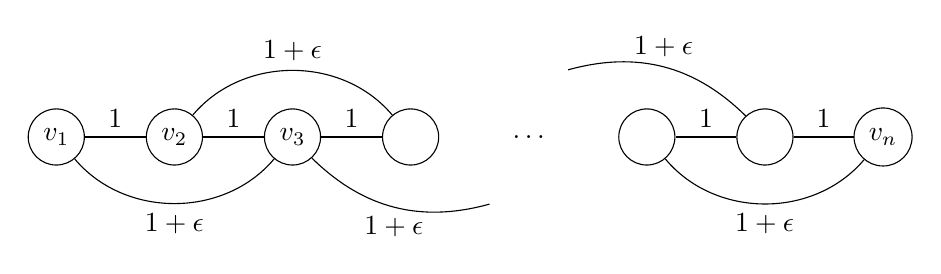
\begin{tikzpicture}[scale=1.5]
			\node[draw, circle] (1) at (0,0) {$v_1$};
			\node[draw, circle] (2) at (1,0) {$v_2$};
			\node[draw, circle] (3) at (2,0) {$v_3$};
			\node[draw, circle] (4) at (3,0) {\phantom{$v_1$}};
			\node (4.5) at (4,0) {$\dots$};
			\node (up) at (4.25, 0.55) {};
			\node (down) at (3.75, -0.55) {};
			\node[draw, circle] (5) at (5,0) {\phantom{$v_1$}};
			\node[draw, circle] (6) at (6,0) {\phantom{$v_1$}};
			\node[draw, circle] (7) at (7,0) {$v_n$};
			
			\draw[-] (1) to node[midway, above] {$1$} (2);
			\draw[-] (2) to node[midway, above] {$1$} (3);
			\draw[-] (3) to node[midway, above] {$1$} (4);
			\draw[-] (5) to node[midway, above] {$1$} (6);
			\draw[-] (6) to node[midway, above] {$1$} (7);
			
			\draw[-, bend right=50] (1) to node[midway, below] {$1 + \epsilon$} (3);
			\draw[-, bend right=50] (5) to node[midway, below] {$1 + \epsilon$} (7);
			
			\draw[-, bend right=30] (3) to node[below] {$1 + \epsilon$} (down);
			\draw[-, bend left=30] (up) to node[above] {$1 + \epsilon$} (6);
			
			\draw[-, bend left=50] (2) to node[midway, above] {$1 + \epsilon$} (4);
			
		\end{tikzpicture}
	\end{center}
	
	
	\newpage
	
	Cristophides sceglie il MST, che in questo caso saranno tutti i lati di lunghezza $1$. $T$ prende tutti gli $n-1$ lati di lunghezza $1$, quindi 
	$$\delta (T) = n-1$$
	
	Gli unici vertici di grado dispari sono il primo e l'ultimo, quindi il minimum perfect matching sarà il lato tra $v_1$ e $v_n$, il quale sarà pari al cammino minimo tra i due ovvero tutti gli $1 + \epsilon$ possibili, più l'ultimo lato:
	$$ \delta(M) = (1 + \epsilon) \frac{n}{2} + 1$$
	
	Il cammino hamiltoniano coinciderà con quello euleriano quindi:
	$$ \delta = \delta (T) + \delta (M) = n-1 + (1 + \epsilon) \frac{n}{2} + 1 = \frac{3}{2} n + \epsilon \frac{n}{2} $$
	
	Ma il circuto ottimo è prendere due lati da 1 affianco a primo ed ultimo nodo, poi tutti i lati da $1 + \epsilon$, quindi il totale: 
	$$ \delta^\ast = (1+ \epsilon)n + 2 $$
	
	Quindi il rapporto di approssimazione diventa: 
	$$ \frac{\delta}{\delta^\ast} = \frac{\frac{3}{2}n + \epsilon \frac{n}{2}}{ (1 + \epsilon) n + 2} \rightarrow \frac{3}{2}$$
	Tende a $3/2$ per $n \rightarrow +\infty$ e $\epsilon \rightarrow 0$.\\
\end{proof}

\newpage

% End L10

\subsubsection{Inapprossimabilità del TSP}

TSP Metrico è approssimabile, \textbf{quello generale no}.\\

\addcontentsline{toc}{subsubsection}{\protect\numberline{}Teorema}
\paragraph{Teorema:} Non esiste $\alpha>1$ tale che TSP sia $\alpha$-approssimabile (se $\mathcal{P} \neq \mathcal{NP}$). Il problema sta fuori da APX.\\

\begin{proof}
	Fact: Il problema di \textbf{decidere se un grafo ammetta un circuito hamiltoniano} è $\mathcal{NP}$-Completo (problema di decisione).\\
	
	Supponiamo per assurdo di \textbf{avere un algoritmo $\alpha$-approssimante per TSP}. \\
	
	Supponendo di avere un grafo $G=(V,E)$ e voler sapere se questo grafo ha un circuito hamiltoniano. Per \textbf{trasformarlo in un'istanza di TSP}, dobbiamo \textbf{aggiungere pesi} e \textbf{trasformarlo in una clique}
	$$ G' = \left(V, \left(
	\begin{array}{c}
		V\\
		2
	\end{array}
	\right), d \right)$$
	
	Bisogna aggiungere le \textbf{distanze}, dove
	$$ 
	d(x,y) = \begin{cases}
		1 & \text{ se } \; \{x,y\} \in E \\
		\lceil \alpha n \rceil + 1 & \text{ altrimenti}
	\end{cases}
	$$
	
	Si tratta di una clique, quindi per forza c'è un circuito hamiltoniano su $G'$, ma se $G$ \textbf{ammetteva} un circuito hamiltoniano allora $G'$ ne B $\leq n$.\\
	Se $G$ \textbf{non ha un circuito hamiltoniano}, qualunque circuito hamiltoniano viene trovato \textbf{su} $G'$ ha \textbf{lunghezza} $\geq \lceil \alpha n\rceil + 1$.\\
	
	\newpage
	
	Diamo $G'$ come \textbf{input dell'algoritmo} $\alpha$-approssimante per TSP, questo \textbf{emetterà} nei casi:
	\begin{itemize}
		\item $G$ ha un c.H.: l'algoritmo emette un output $\leq \alpha n$ (dato che si tratta di una $\alpha$-approssimazione)
		\item $G$ non ha un c.H.: l'algoritmo emette un output $\geq \lceil \alpha n \rceil + 1$
	\end{itemize}
	
	Quindi possiamo avere output $\leq \alpha n$ e  $\geq \lceil \alpha n \rceil + 1$, ma \textit{è possibile che questi due intervalli si sovrappongano}?
	$$ \alpha n \geq \lceil \alpha n \rceil + 1 $$
	$$ \implies \alpha \geq \frac{\lceil \alpha n \rceil + 1}{n} \geq \frac{\alpha n + 1}{n} = \alpha + \frac{1}{n}$$
	$$ \alpha \geq \alpha + \frac{1}{n}$$
	
	Quindi sono \textbf{intervalli sempre disgiunti} e di conseguenza le soluzioni sono ben distinte.\\
	
	Questo vorrebbe dire risolvere il problema di decidere se un grafo ammetta un circuito hamiltoniano efficientemente, che sappiano non essere possibile essendo in $\NP$.\\
\end{proof}

\newpage

\section{Schemi di approssimazione PTAS e FPTAS}
\subsection{PTAS per 2-LoadBalancing}

Ricordando cos'è un PTAS: problemi approssimabile a meno di una costante desiderata (arriva al tasso di approssimazione desiderato).\\

LoadBalancing già visto, quello delle macchine e task, bla bla bla. 2-LoadBalancing è la stessa cosa ma ha \textbf{solo 2 macchine}.\\

\textbf{Definizione} del problema:
\begin{itemize}
	\item \textbf{Input}: sequenza di $n$ task $t_0, \, \dots \, , t_{n-1}$
	\item \textbf{Soluzioni ammissibili}: assegnamenti dei task su 2 macchine, una funzione $\alpha: n \rightarrow 2$
	\item \textbf{Funzione obiettivo}: massimo carico tra le due macchine 
	$$ \max \left(\sum_{i: \alpha(i)=0} t_i , \sum_{i: \alpha(i)=0} t_a\right) $$
	\item \textbf{Tipo}: minimizzazione, $\min$
\end{itemize}

\nn

Per l'\textbf{algoritmo PTAS}: 
\begin{itemize}
	\item \textbf{Input}:  i task $t_0, \, \dots \, , t_{n-1}$ ed un \textbf{costante di approssimazione} (circa) $\epsilon > 0$ (per avere una $1+\epsilon$-approssimazione)
\end{itemize}

\newpage

\paragraph{Passaggi:}
\begin{itemize}
	\item If $\epsilon \geq 1$: 
	\begin{itemize}
		\item Assegna tutti i task alla prima macchina 
		\item Termina
	\end{itemize}
	\nn
	
	\item Altrimenti, ordina i $t_i$ in \textbf{ordine decrescente}.\\
	
	\item \textbf{Fase 1}:
	\begin{itemize}
		\item \textbf{Calcola} $k \leftarrow \lceil \frac{1}{\epsilon} -1 \rceil$
		\item Si \textbf{cerca esaustivamente} l'assegnamento ottimo dei task $t_0, \, \dots \, , t_{k-1}$ (primi $k$ task, $2^k$ assegnamenti possibili)
	\end{itemize}
	\nn
	
	\item \textbf{Fase 2}:
	\begin{itemize}
		\item I \textbf{restanti task}  $t_k, \, \dots \, , t_{n-1}$ sono \textbf{assegnati} in modo \textbf{greedy} (sempre alla macchina più scarica)
	\end{itemize}
	\nn
\end{itemize}

L'assegnamento dei task "grossi" (i primi) viene risolto a forza bruta, il resto greedy.\\

\addcontentsline{toc}{subsubsection}{\protect\numberline{}Teorema}
\paragraph{Teorema:} l'algoritmo è una $(1+ \epsilon)$-approssimazione di $2$-LoadBalancing.\\

\begin{proof}
	Chiamando la \textbf{somma dei task}
	$$ T := \sum_{i \in n} t_i$$
	
	Se $\epsilon \geq 1$, otteniamo una 2-Approssimazione (butto tutto su una, di sicuro non può essere peggio di 2 volte la soluzione ottima).
	$$ L^\ast \geq \frac{T}{2}, \;\;\;\;\; L = T $$
	$$\implies \frac{L}{L^\ast} \leq \frac{T}{\sfrac{T}{2}}$$
	
	Nel caso in cui $\epsilon < 1$: alla \textbf{fine della prima fase} abbiamo l'\textbf{assegnamento ottimo} per i primi $k$ task ed un carico sulle macchine 0 e 1, rispettivamente $y_0$ e $y_1$. \\
	
	Rimangono \textbf{da assegnare} i task $t_k, \, \dots \, , t_{n-1}$ per arrivare agli \textbf{assegnamenti finali} $L_0$ e $L_1$.\\
	
	Assumiamo (senza perdita di generalità) che $L_0 \geq L_1$ (\textbf{alla fine} la macchina con il \textbf{carico maggiore} è \textbf{la prima}).\\
	
	Due casi: 
	\begin{enumerate}
		\item $L_0 = y_0$, dopo la prima fase tutti i restanti task sono stati attribuiti alla seconda macchina.\\
		$\implies$ abbiamo \textbf{ottenuto l'assegnamento ottimo}, per costruzione dell'algoritmo.\\
		
		\item Uno o più task di $t_k, \, \dots \, , t_{n-1}$ sono stati assegnati alla prima macchina, sia $t_h$ l'\textbf{ultimo assegnato} a suddetta macchina (il più piccolo). Di conseguenza
		$$ L_0 - t_h \leq L_1' \leq L_1$$
		
		(dove $L_1'$ è il carico della seconda macchina prima dell'assegnamento di $t_h$). Ovviamente prima di assegnare $t_h$ il carico sulla prima macchina era minore del carico sulla seconda macchina
		$$ \implies 2L_0 - t_h \leq L_0 + L_1 $$
		$$ T = L_0 + L_1$$
		$$ \implies L_0 - \frac{t_h}{2} \leq \frac{T}{2} $$
		$$ L_0 \leq \frac{T}{2} + \frac{t_h}{2} $$
		
		Ricordiamo che \textbf{i primi $k$ task sono} $\geq (k+1) t_h$, in quanto ordinati in ordine decrescente
		$$ T \geq (k+1) t_h $$
		
		I task dopo $t_h$ li minoriamo con 0.
		$$ \frac{T}{2} \geq (k+1) \frac{t_h}{2} $$
		
		\textbf{Quindi}
		$$ \frac{L_0}{L^\ast} \leq \frac{L_0}{\sfrac{T}{2}} \leq \frac{\frac{T}{2} + \frac{t_h}{2}}{\sfrac{T}{2}} = 1 + \frac{t_h}{T} \leq 1 + \frac{t_h}{(k+1) t_h} = 1 + \frac{1}{(k+1)} $$
		
		Ma \textbf{per definizione di} $k$ 
		$$ \frac{L_0}{L^\ast} \leq 1 + \frac{1}{(k+1)} \leq 1 + \frac{1}{\frac{1}{\epsilon} - 1 + 1} = 1 + \epsilon $$
	\end{enumerate}
	$$ \implies  \frac{L_0}{L^\ast} \leq 1 + \epsilon $$
\end{proof}

\addcontentsline{toc}{subsubsection}{\protect\numberline{}Teorema}
\paragraph{Teorema:} Il PTAS \textbf{richiede tempo} $O\left(n \log n + 2^{\min \left(\frac{1}{\epsilon}, n\right)}\right)$.\\

\begin{proof}
	$n \log n$ è il \textbf{tempo} per l'\textbf{ordinamento}.\\
	
	L'\textbf{esponenziale} è la \textbf{fase di assegnamento esatto}.\\
	
	Abbiamo $2^k$ assegnamenti ma 
	$$ 2^k = 2^{\lceil \frac{1}{\epsilon} - 1\rceil} \sim 2^{\frac{1}{\epsilon}}$$
	
	Ci sarebbe anche la parte di assegnamento greedy ma talmente breve che non conta.\\
\end{proof}

Quindi abbiamo un algoritmo PTAS, con un \textbf{tasso di approssimazione arbitrariamente preciso} ma con \textbf{tempo che peggiora esponenzialmente} in base a quest'ultimo.\\

\newpage

\subsection{Knapsack Problem}

I pirati arrivano in una grotta con degli oggetti, ognuno di questi $n$ oggetti ha un valore 
$$ v_0, \, \dots \, , v_{n-1} $$

ed i pirati vogliono portarsi a casa il maggior valore possibile, ma per portarli hanno solo uno zaino con una capacità $W$ ed ogni oggetto ha un peso  
$$ w_0, \, \dots \, , w_{n-1} $$

I pirati vogliono portare a casa il maggior valore possibile con un peso che rientra nello zaino.\\

% End L11

\paragraph{Definizione del problema: }
\begin{itemize}
	\item \textbf{Input}: $n>0$ numero di oggetti, $v_i, w_i \in \mathbb{N}^+$ valori e pesi associati agli oggetti, $i <n$, capacità dello zaino $W>0$
	\item \textbf{Soluzioni ammissibili}: $X \subseteq n$ tale che 
	$$ \sum_{i \in X} w_i \leq W $$
	\item \textbf{Funzione obiettivo}: la somma dei valori 
	$$v = \sum_{i \in X} v_i$$
	\item \textbf{Tipo}: massimizzazione, $\max$
\end{itemize}

\newpage

\paragraph{Side quest: Programmazione Dinamica:} vogliamo risolvere un certo problema $\pi$, nel quale sono presenti dei parametri $\pi [\overline{a},\overline{b}]$, ma il problema si può presentare in varianti con valori diversi da $\overline{a}$ e $\overline{b}$.\\

Voglio poter \textbf{risolvere} una certa \textbf{istanza di un problema a partire da istanze precedenti}/più semplici/con valori più semplici risolte in precedenza.\\
Devo quindi risolvere soluzioni più semplici per arrivare a quelle più grosse, le soluzioni dipendono da quelle prima.\\

Il numero di problemi da risolvere prima della soluzione che cerco è pari a tutte le possibili combinazioni di valori di parametri fino a $\overline{a}$ e $\overline{b}$. Si possono pensare le diverse istanze da risolvere come se fossero in una tabella con da un lato tutti i valori possibili del parametro $\overline{a}$ e dell'altro i possibili valori di $\overline{b}$.

$$
\begin{array}{c | c | c | c | c }
	& 0 & 1 & \dots & \overline{a} \\
	\hline
	0 & & & & \\
	\hline
	1 & & & & \\
	\hline
	\dots & & & & \\
	\hline
	\overline{b} & & & &
\end{array}
$$

In ognuna delle celle la soluzione dell'istanza di $\pi$ con i relativi valori dei parametri.\\

Fondamentale i parametri siano valori interi, altrimenti si può risolvere tutto in tempo polinomiale.\\

\paragraph{Side-side-quest: pseudopolinomialità:} Un algoritmo è pseudopolinomiale quando il suo \textbf{tempo di esecuzione dipende dal valore numerico degli input} considerati, al posto che dalla grandezza della rappresentazione. Un valore $n$ in binario richiede $b = \lceil \log_2 n \rceil$ bit, ma il valore considerato è $n \leq 2^b$, quindi il tempo d'esecuzione è esponenziale rispetto alla dimensione dell'input.\\

\newpage

\subsubsection{Soluzione di Programmazione Dinamica: Versione A}

Partendo dalle $n$ coppie di valori-pesi.\\

I parametri secondo cui iterare con la programmazione dinamica (righe e colonne della tabella) sono: 
\begin{itemize}
	\item $W$, \textbf{capienza dello zaino}, risolvo il problema per tutti i valori da 0 a $W$
	\item \textbf{Numero di oggetti}, considero solo i primi $i$ oggetti, variando il valore di $i$ tra 0 e $n$
\end{itemize}

Posso costruire una tabella con in \textbf{ogni riga tutte le soluzione per un possibile valore per la capienza dello zaino} $W$ e la colonna $i$ contiene le soluzioni considerando solo i primi $i$ oggetti. Quindi la cella $3,2$ contiene il valore massimo ottenibile con i primi $3$ oggetti e capienza $2$.\\

\textbf{Ogni cella} della tabella contiene il valore massimo che i pirati si portano a casa, i.e., il risultato del problema, i.e., il \textbf{valore della funzione obiettivo}.\\

La prima riga, non importa  quanti oggetti considero, se lo zaino ha capienza 0 non posso metterci nulla.\\
La prima colonna anch'essa è tutti zero, in quanto non ho oggetti, anche con un camion al posto dello zaino nella grotta non trovo nulla.\\

Quindi come posso trovare il \textbf{valore} $v(w,i)$ \textbf{per una qualsiasi cella?} Presupponendo di riempire la tabella da sinistra verso destra, dall'alto verso il basso. La $w$ rappresenta la capienza considerata, la funzione $v$ rappresenta il valore portato a casa e la $i$ indica che abbiamo considerato i primi $i$ oggetti, quelli che hanno da indice 0 a $i-1$.\\

Guardo \textbf{i valori precedenti}, partendo da $v(w,i-1)$:
\begin{itemize}
	\item Se decido di non aggiungere l'$i$-esimo elemento il risultato non cambia, in quanto ho già trovato il risultato migliore per quello stesso spazio
	\item Altrimenti, se voglio aggiungere l'$i$-esimo elemento con valore $v_i$, aggiungo il suo valore, ma lo zaino deve essere abbastanza capiente
\end{itemize}

Formalmente:
$$
v (w,i) = \begin{cases}
	v (w, i-1) & \text{ se } w < w_{i-1} \\
	\max \left(v(w,i-1), v_{i-1} + v (w - w_{i-1}, i-1)\right) & \text{ altrimenti }
\end{cases}
$$
Quindi, se non c'è abbastanza spazio ($w < w_{i-1}$) per aggiungere l'$i$-esimo elemento il valore rimane lo stesso.\\

Altrimenti prendo il massimo tra il valore della cella subito a sinistra e il valore della migliore cella la cui capienza associata mi permette di aggiungere l'$i$-esimo elemento.\\

Il numero di colonne è $n$, ma tutti i possibili valori di $W$ sono pseudo-polinomiali $\implies$ complessità esponenziale.\\

\newpage

\subsubsection{Soluzione di Programmazione Dinamica: Versione B}

Tengo la nostra tabella per la programmazione dinamica, in riga sempre il numero di oggetti considerati, ma \textbf{in colonna metto il valore che i pirati vogliono portarsi a casa}, di conseguenza \textbf{nelle celle} calcolo \textbf{la minima capacità di uno zaino per ottenere quel valore}. Stesso problema, stiamo solo cambiando la rappresentazione.\\

Se il valore obiettivo è 0, la dimensione necessaria è sempre 0, si tratta di un pirata molto umile.\\
Se voglio portare a casa un valore $>0$, ma sto considerando $0$ elementi risulta difficile $\implies$ la prima colonna è tutta $+ \infty$ (tranne la prima cella a zero).\\

Come ottengo \textbf{una cella qualunque} $w(v,i)$?\\

Se decido di non portare a casa anche l'$i$-esimo oggetto rimane tutto come $w(v, i-1)$, altrimenti diventa $w_{i-1} + w (v - v_{i-1}, i-1)$, quindi
$$ w (v,i) = \begin{cases}
	\min \left(w (v, i-1), w_{i-1}\right) & \text { se } v < v_{i-1} \\
	\min \left(w (v, i-1), w_{i-1} + w (v - v_{i-1}, i-1) \right) & \text{ altrimenti }
\end{cases}$$
Se il valore cercato è minore del valore dell'oggetto che ho appena introdotto posso scegliere di prendere solo quest'ultimo.\\

Altrimenti prendo il minimo tra il valore subito a sinistra e la somma tra il peso dell'$i$-esimo oggetto e il peso della cella contenente il valore minimo necessario per arrivare al nostro obiettivo una volta sommato il valore dell'oggetto appena inserito.\\

Quindi, compilo la tabella, ma \textbf{avrò delle celle in cui il peso minimo è too much}, $> W$, l'\textbf{output} per il nostro problema lo \textbf{ottengo risalendo} dalla cella in basso a destra verso l'alto \textbf{finché non trovo un valore di capienza minima ammissibile} $w < W$, i.e., prendo il valore ammissibile più alto possibile.\\

\newpage

\subsubsection{Algoritmo DP Approssimato}

Problema: gli algoritmi precedenti sono esatti, ma sono entrambi esponenziali nel numero di righe.\\

Per \textbf{approssimare il problema} possiamo "\textit{comprimere le righe}", ovvero \textbf{dividiamo tutti i valori per un certo numero}, \textbf{diminuendo} così il \textbf{numero di righe} necessarie, fino a far diventare l'algoritmo polinomiale.\\

Si può fare \textbf{solo con la seconda versione}, in cui le righe rappresentano la funzione obiettivo (che possiamo approssimare, andando ad ottenere un sub-ottimo), mentre con la prima versione non possiamo comprimere la capacità dello zaino, in quanto parte dei constraint del problema, rischieremmo di andare verso soluzioni non ammissibili.\\

Quindi, applichiamo il secondo algoritmo, ma con \textbf{scaling}.\\

Al problema $\pi (v_i, w_i, W)$ aggiungiamo $\epsilon \in (0,1]$ e vogliamo una \textbf{$(1+\epsilon)$-approssimazione} di $\pi$
$$ \theta = \frac{\epsilon \cdot v_{max}}{2n}$$

Aggiungiamo \textbf{due ulteriori versioni del problema}: 
$$ \overline{\pi} \left(\overline{v}_i = \left\lceil \frac{v_i}{\theta} \right\rceil \theta, w_i, W\right) $$

Quindi arrotondo un po' i valori per eccesso, mentre in 
$$ \hat \pi = \left( \hat v_i = \left\lceil \frac{v_i}{\theta} \right\rceil, w_i, W \right)$$
approssimo ma lascio compresso, quindi noi vogliamo risolvere $\hat \pi$ in modo esatto tramite il secondo algoritmo di programmazione dinamica visto precedentemente.\\

\newpage

Dobbiamo capire \textbf{come sono correlate le tre soluzioni}:
$$ \hat X^\ast \subseteq n, \;\;\;\; \overline X^\ast \subseteq n \;\;\;\; X^\ast \subseteq n$$

\paragraph{Osservazione:} l'\textbf{ammissibilità è la stessa} per tutti e 3 i problemi, tutti i problemi hanno le stesse soluzioni ammissibili.\\

\paragraph{Osservazione:} Le soluzioni 
$$ \hat X^\ast = \hat X^\ast$$
in quanto sono problemi uguali, i valori sono solo moltiplicati per una costante. \textbf{Queste soluzioni sono uguali}.\\

\paragraph{Lemma:} Sia $X$ una soluzione ammissibile, 
$$ (1 + \epsilon) \sum_{i \in \hat X^\ast} v_i \geq \sum_{i \in X} v_i $$
La soluzione ottima dei nostri problemi modificati, moltiplicata per la costante di approssimazione, è sempre $\geq$ di qualsiasi soluzione ammissibile.\\

\begin{proof}
	Dato che $\hat \pi$ ha degli arrotondamenti per eccesso, tutti i valori saranno un po' più grandi, quindi 
	$$ \sum_{i \in X} v_i \leq \sum_{i \in X} \hat v_i \leq \sum_{i \in \overline X^\ast} \hat v_i $$
	E ovviamente, la soluzione ottima per $\hat \pi$ ha un valore maggiore di una qualsiasi soluzione ammissibile.\\
	
	%\newpage
	
	Per come sono definiti 
	$$\hat v_i - v_i \leq \theta $$
	
	Quindi 
	$$ \sum_{i \in \overline X^\ast} \hat v_i 
	\leq \sum_{i \in \overline X^\ast} (v_i + \theta) 
	= \sum_{i \in \overline X^\ast} v_i + |\overline X^\ast| \theta \leq $$
	$$\leq \sum_{i \in \overline X^\ast} v_i + n \theta 
	= \sum_{i \in \overline X^\ast} v_i + n \frac{\epsilon \cdot v_{max}}{2n}
	$$ 
	
	Quindi 
	$$ \sum_{i \in X} v_i \leq \sum_{i \in \overline X^\ast} v_i + \frac{\epsilon \cdot v_{max}}{2} $$
	è vera per ogni soluzione ammissibile $X$.\\
	
	Prendo solo l'indice dell'elemento del valore massimo:
	$$ X = \{i_{max}\}$$
	(ovviamente escludendo gli elementi con $w_i>W$).\\
	
	Questa è una soluzione ammissibile, quindi
	$$ v_{max} \leq \sum_{i \in \overline X^\ast} v_i + \frac{\epsilon \cdot v_{max}}{2} \leq  $$
	Essendo $\epsilon \leq 1$
	$$\leq  \sum_{i \in \overline X^\ast} v_i + \frac{v_{max}}{2}$$
	$$ \implies \frac{v_{max}}{2} \leq \sum_{i \in \overline X^\ast} v_i $$
	
	Quindi la disuguaglianza precedente
	$$ \sum_{i \in X} v_i \leq \sum_{i \in \overline X^\ast} v_i + \frac{\epsilon \cdot v_{max}}{2} $$
	diventa
	$$ \sum_{i \in X} v_i \leq (1 + \epsilon) \sum_{i \in \overline X^\ast} v_i$$
	
	Ma ricordando che $\hat X^\ast = \overline X^\ast$
	$$ \sum_{i \in X} v_i \leq (1 + \epsilon) \sum_{i \in \hat X^\ast} v_i $$
\end{proof}

\newpage

\addcontentsline{toc}{subsubsection}{\protect\numberline{}Teorema}
\paragraph{Teorema:} Il lemma vale per tutte le soluzioni, anche quella originale
$$(1 + \epsilon) \hat v^\ast \theta \geq v^\ast$$

\begin{proof}
	Il Lemma dice che
	$$ (1 + \epsilon) \sum_{i \in \hat X^\ast} v_i \geq \sum_{i \in X} v_i $$
	Ma la prima parte è $\leq \hat v^\ast \theta$ e la seconda è una qualsiasi soluzione ammissibile, quindi anche $X^\ast$ e di conseguenza $v^\ast$.\\
\end{proof}

Non sono un cazzo sicuro di questo teorema ma trust me bro.\\

Comprimo i valori, faccio i miei calcoli, ma poi alla fine devo decomprimerli per sapere il mio risultato, per questo ho il $\theta$ in giro, la discrepanza è data dall'approssimazione per eccesso effettuata.\\

\paragraph{Corollario:} L'algoritmo è una \textbf{$(1 + \epsilon)$-approssimazione}.\\

\paragraph{Complessità:} devo guardare le celle della tabella, ovvero il numero di colonne per il numero di righe, quindi 
$$ n \cdot \sum \hat v_i \leq n^2 \hat v_{max} = n^2 \left\lceil \frac{v_{max}}{\theta} \right\rceil = $$
$$ = n^2 \left\lceil \frac{2 v_{max} n}{\epsilon \cdot v_{max}} \right\rceil = O\left(\frac{n^3}{\epsilon}\right) $$
la disuguaglianza è data dal fatto che ognuno degli $n$ elementi è per forza minore del massimo $v_{max}$

In totale quindi diventa
$$ O \left(\frac{n^3}{\epsilon}\right)$$
Ovvero, polinomiale in $n$ e in $\epsilon$, quindi \textbf{è un FPTAS}.\\

\newpage

%End L12